\documentclass[12pt]{article}
\setlength{\oddsidemargin}{0in}
\setlength{\evensidemargin}{0in}
\setlength{\textwidth}{6.5in}
\setlength{\parindent}{0in}
\setlength{\parskip}{\baselineskip}

\usepackage{amsmath,amsfonts,amssymb,graphicx,xcolor,mathtools}

\newcommand{\purple}[1]{{\color{purple} #1}}

\begin{document}

PHYS 374 Fall 2020\hfill Worksheet 7: The Ramp is Fixed This Time\\
\\
Name:\\
\\
Please submit as a PDF on Moodle. Include any calculations made using external tools.

\hrulefill
\\
\\
A ball rolls without slipping down a ramp of angle $\theta$. The ramp is fixed. 

\begin{enumerate}
\item Draw a picture!
\item Write down the Lagrangian for this system in terms of $x$ (the position of the ball) and $\phi$ (the ball's rotation). Recall that the rotational kinetic energy of a sphere is:
$$
T_{rot} = \tfrac{1}{2} I \dot{\phi}^2
\quad\quad\text{where $I=\tfrac{2}{5}mr^2$ for a sphere rotating around its center}
$$
\item What is the relationship between $x$ and $\phi$ for the ball to roll without slipping?

Hint: constraints should take the form $g(x, \phi) = \text{const}$
\item Use the Euler-Lagrange equation with a Lagrange multiplier $\lambda$ to get the equations of motion for the system.
$$
\frac{\partial \mathcal{L}}{\partial x} + \lambda \frac{\partial g}{\partial x} = \frac{d}{dt} \frac{\partial \mathcal{L}}{\partial \dot{x}}
\quad\quad\text{and likewise for $\phi$}
$$
\item Use your equations of motion and your constraint to solve for $\ddot{x}$. How does it compare to the acceleration of a block sliding down a frictionless ramp? 
\item What is the value of the Lagrange multiplier $\lambda$? What is its physical significance?

\end{enumerate}

\newpage

\purple{

\begin{figure}[h]
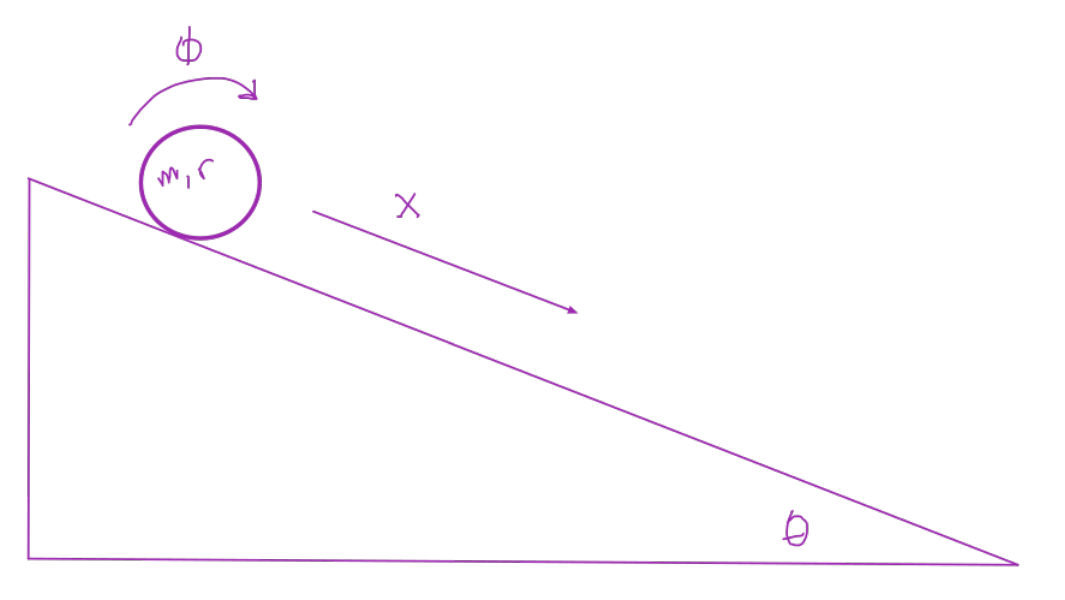
\includegraphics[width=5cm]{rolling-down-ramp.png}
\centering
\end{figure}

Kinetic energy has a translational term and a rotational term. Potential energy is just gravity.
$$
T = \tfrac{1}{2} m \dot{x}^2 + \tfrac{1}{2} I \dot{\phi}^2
\quad\quad\text{and}\quad\quad
U = mgy = -mg x \sin \theta
$$
So the Lagrangian is:
$$
\mathcal{L} = \tfrac{1}{2} m \dot{x}^2 + \tfrac{1}{2} I \dot{phi}^2 + mg x \sin \theta
$$
The ball is rolling without slipping, so the distance moved by the ball must match up with the distance its surface rolls:
$$
x = r \phi
\quad\quad\rightarrow\quad\quad
x - r\phi = \text{const}
$$
Plugging into the Euler-Lagrange equation we get (for $x$ and $\phi$ respectively):
$$
mg\sin\theta + \lambda = m\ddot{x}
\quad\quad\text{and}\quad\quad
-r\lambda = I \ddot{\phi}
$$
We then get a relationship between $\ddot{x}$ and $\ddot{\phi}$ by differentiating our constraint equation:
$$
x = r \phi
\quad\quad\rightarrow\quad\quad
\dot{x} = r\dot{\phi}
\quad\quad\rightarrow\quad\quad
\ddot{x} = r\ddot{\phi}
$$
After a bit of finagling, and substituting $I=\tfrac{2}{5} m r^2$, we find:
$$
\ddot{x} = \tfrac{5}{7} g \sin\theta
$$
For comparison, an object sliding down a frictionless ramp does so at $g\sin\theta$. A rolling object moves slower. One way to think about it is that, when sliding, all gravitational energy becomes translational energy. When rolling, some of it becomes rotational energy instead. 

Another perspective is friction! In order to gain angular velocity, there must be a torque on the ball about its center of mass. Gravity acts on the center of mass, and so provides no torque. Friction with the surface, a force that points in the $-\hat{x}$ direction, is what provides the torque. 

In general, friction comes with energy loss. In the case of rolling without slipping, there is no energy loss because the frictional force does no work -- the point it's acting on does not slip.

}
\end{document}